\section{代码布局(Code Layout)}

\begin{frame}[fragile]
    \frametitle{什么是代码布局}
    指令连续地、有顺序地储存在内存中。LLVM中,这些优化过程抽象成控制流图中的基本块(Basic Block, BB)的排列方式。

    \begin{columns}
        \begin{column}{0.2\textwidth}
            \centering
            C Codes:
            \begin{lstlisting}
if (a < b)
    c = 1;\end{lstlisting}
        \end{column}
        \begin{column}{0.5\textwidth}
\begin{lstlisting}[language={[RISC-V]Assembler}]
; a is in a0
; b is in a1
; c is in a2
bge a0 a1 .LBB0_2
j .LBB0_1
li a2 1
.LBB0_2:\end{lstlisting}
        \end{column}
    \end{columns}
\end{frame}

\begin{frame}
    \frametitle{机器代码布局优化}
    基于机器相关的,代码布局的优化主要包含,基本块放置(Basic block placement)、基本块对齐(Basic block alignment)、冷热代码分离(Hot-Cold Splitting)\cite{bakhvalov-2019}.
    \begin{figure}
        \centering
        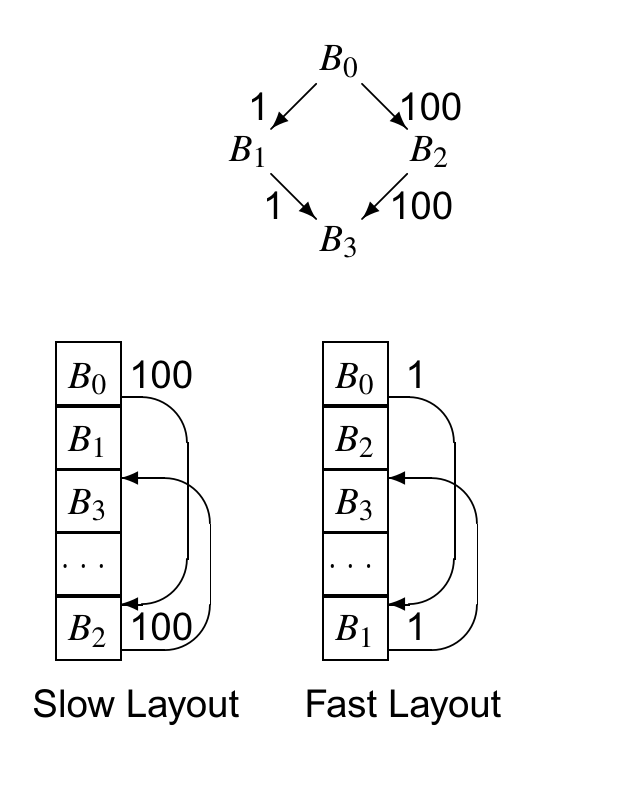
\includegraphics[width=0.21\textwidth]{images/layout_compare.png}
        \caption{两种不同布局的优劣\cite{cooper2011engineering}}
    \end{figure}

\end{frame}


\begin{frame}[fragile]
\frametitle{基本块放置 - Basic Block Placement}

    \begin{columns}
        \begin{column}{0.3\textwidth}
            \centering
            C Codes:
            \begin{lstlisting}
// hot path
if (cond)
    coldFunc();
// hot path again\end{lstlisting}
        \end{column}
        \begin{column}{0.65\textwidth}
            \begin{figure}
                \centering
                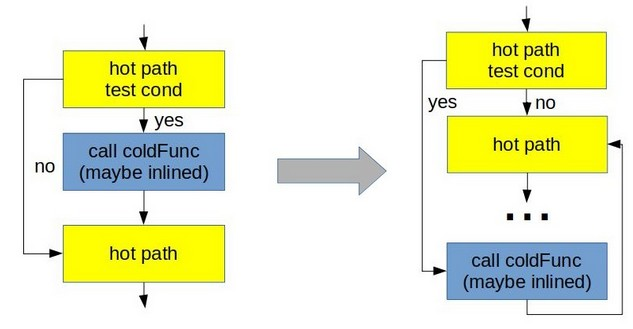
\includegraphics[width=0.86\textwidth]{images/hot_cold_placement.jpg}
                \caption{布局优化示例}
            \end{figure}
        \end{column}
    \end{columns}
    \begin{itemize}
        \item 不进行分支跳转往往比跳转代价更低(maintain fall through)
        \item 更好地利用 Cache ($\mu$op-cache) (局部性)
    \end{itemize}

\end{frame}

\begin{frame}
\frametitle{基本块对齐 - Basic Block Alignment}
\centering

A brief explanation of the manner:

\begin{figure}
    \centering
    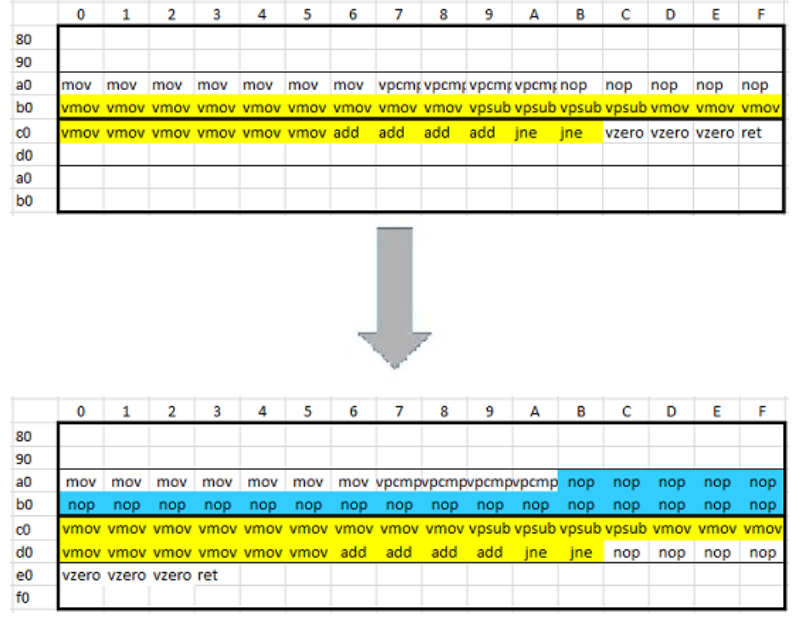
\includegraphics[width=0.418\textwidth]{images/alignment.png}
    \caption{基本块对齐}
\end{figure}

\end{frame}
\begin{frame}[fragile]
    \frametitle{冷热代码分离 - 分离前}
    冷热代码分离的核心思想是,将冷代码(如错误处理)分成一个独立的函数调用,从原过程(procedure)中分离,然后用一个函数调用语句代替冷代码,从而提高热代码的连续性、局部性。
    \begin{columns}
        \begin{column}{0.7\textwidth}
            \begin{lstlisting}
void foo(bool cond1, bool cond2) {
    // hot path
    if (cond1)
        // cold code 1
    //hot code
    if (cond2)
        // cold code 2
}
            \end{lstlisting}
        \end{column}
    \end{columns}
\end{frame}


\begin{frame}[fragile]
    \frametitle{冷热代码分离 - 分离后的代码}
    \begin{columns}
        \begin{column}{1.0\textwidth}
            \begin{lstlisting}
void foo(bool cond1, bool cond2) {
    // hot path
    if (cond1)
        cold1(); 
    //hot code
    if (cond2)
        cold2(); 
    }
    
    void cold1() __attribute__((noinline)) { // cold code 1 }
    void cold2() __attribute__((noinline)) { // cold code 2 }
            \end{lstlisting}
        \end{column}
    \end{columns}
\end{frame}

\begin{frame}
    \frametitle{冷热代码分离 - 图}
这样做的好处是,热指令都会存在同一个cache line里,可以提高CPU前端数据结构的利用效率,例如I-cache 和 DSB-Cache
    \begin{figure}
        \centering
        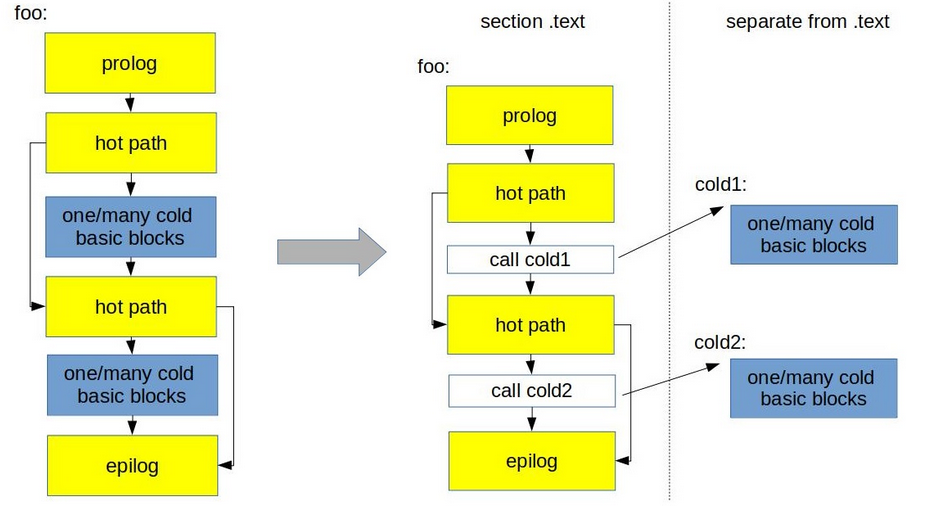
\includegraphics[width=0.63\textwidth]{images/splitting.png}
\caption{将冷代码过程转换为函数调用}
    \end{figure}

\end{frame}